\section{GAMMALN Log Gamma Function}

\subsection{Usage}

Computes the natural log of the gamma function for real arguments.  The \verb|gammaln|
function takes only a single argument
\begin{verbatim}
  y = gammaln(x)
\end{verbatim}
where \verb|x| is either a \verb|float| or \verb|double| array.  The output
vector \verb|y| is the same size (and type) as \verb|x|.
\subsection{Example}

Here is a plot of the \verb|gammaln| function over the range \verb|[-5,5]|.
@>
which results in the following plot.


\centerline{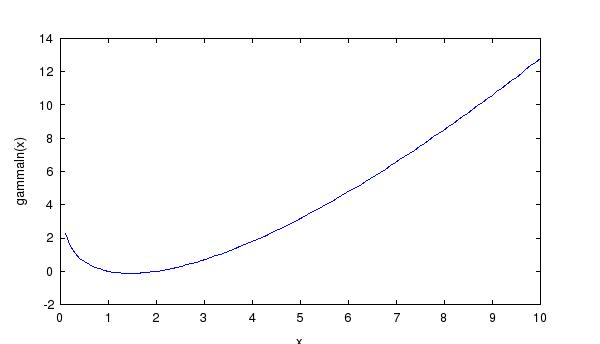
\includegraphics[width=8cm]{gammaln1}}

